\section{AddrMap Class Reference}
\label{classAddrMap}\index{AddrMap@{AddrMap}}
Class for handling adress translations within the Memory Controller =====================================================================================.  


{\tt \#include $<$addr\_\-map.h$>$}

Inheritance diagram for AddrMap:\nopagebreak
\begin{figure}[H]
\begin{center}
\leavevmode
\includegraphics[width=146pt]{classAddrMap__inherit__graph}
\end{center}
\end{figure}
Collaboration diagram for AddrMap:\nopagebreak
\begin{figure}[H]
\begin{center}
\leavevmode
\includegraphics[height=400pt]{classAddrMap__coll__graph}
\end{center}
\end{figure}
\subsection*{Public Member Functions}
\begin{CompactItemize}
\item 
{\bf AddrMap} ()
\begin{CompactList}\small\item\em constructor \item\end{CompactList}\item 
{\bf $\sim$AddrMap} ()
\begin{CompactList}\small\item\em deconstructor \item\end{CompactList}\item 
void {\bf process\_\-event} ({\bf IrisEvent} $\ast$e)
\begin{CompactList}\small\item\em Main function that handles this class. \item\end{CompactList}\item 
void {\bf map\_\-addr} ({\bf Request} $\ast$req)
\begin{CompactList}\small\item\em Main address translation function. \item\end{CompactList}\item 
std::string {\bf toString} ()
\end{CompactItemize}
\subsection*{Public Attributes}
\begin{CompactItemize}
\item 
{\bf Component} $\ast$ {\bf parent}
\begin{CompactList}\small\item\em pointer to the request handler \item\end{CompactList}\end{CompactItemize}


\subsection{Detailed Description}
Class for handling adress translations within the Memory Controller =====================================================================================. 

Description: 

Definition at line 44 of file addr\_\-map.h.

\subsection{Constructor \& Destructor Documentation}
\index{AddrMap@{AddrMap}!AddrMap@{AddrMap}}
\index{AddrMap@{AddrMap}!AddrMap@{AddrMap}}
\subsubsection[{AddrMap}]{\setlength{\rightskip}{0pt plus 5cm}AddrMap::AddrMap ()}\label{classAddrMap_444d016dee4f23d333ce23555fa9a216}


constructor 



Definition at line 34 of file addr\_\-map.cc.\index{AddrMap@{AddrMap}!$\sim$AddrMap@{$\sim$AddrMap}}
\index{$\sim$AddrMap@{$\sim$AddrMap}!AddrMap@{AddrMap}}
\subsubsection[{$\sim$AddrMap}]{\setlength{\rightskip}{0pt plus 5cm}AddrMap::$\sim$AddrMap ()}\label{classAddrMap_160df7459c1afe77115c3f1a22759a15}


deconstructor 



Definition at line 46 of file addr\_\-map.cc.

\subsection{Member Function Documentation}
\index{AddrMap@{AddrMap}!map\_\-addr@{map\_\-addr}}
\index{map\_\-addr@{map\_\-addr}!AddrMap@{AddrMap}}
\subsubsection[{map\_\-addr}]{\setlength{\rightskip}{0pt plus 5cm}void AddrMap::map\_\-addr ({\bf Request} $\ast$ {\em req})}\label{classAddrMap_0da8ea664e351b258473e04935d7170a}


Main address translation function. 



Definition at line 121 of file addr\_\-map.cc.

References addr\_\-map\_\-scheme, Request::address, BANK\_\-BITS, Request::bankNo, BLOCKS\_\-PER\_\-ROW, CACHE\_\-BLOCK\_\-SIZE, CACHELINE\_\-INTERLEAVING, Request::channelNo, COLUMN\_\-SIZE, Request::columnNo, DRAM\_\-SIZE, GENERIC, LOCAL\_\-ADDR\_\-MAP, Request::lowerBits, NO\_\-OF\_\-BANKS, NO\_\-OF\_\-CHANNELS, NO\_\-OF\_\-COLUMNS, NO\_\-OF\_\-RANKS, NO\_\-OF\_\-ROWS, NO\_\-SCHEME, PAGE\_\-INTERLEAVING, PERMUTATION, Request::rankNo, ROW\_\-SIZE, Request::rowNo, SWAPPING, and TAG\_\-BITS.

Referenced by process\_\-event().

Here is the caller graph for this function:\nopagebreak
\begin{figure}[H]
\begin{center}
\leavevmode
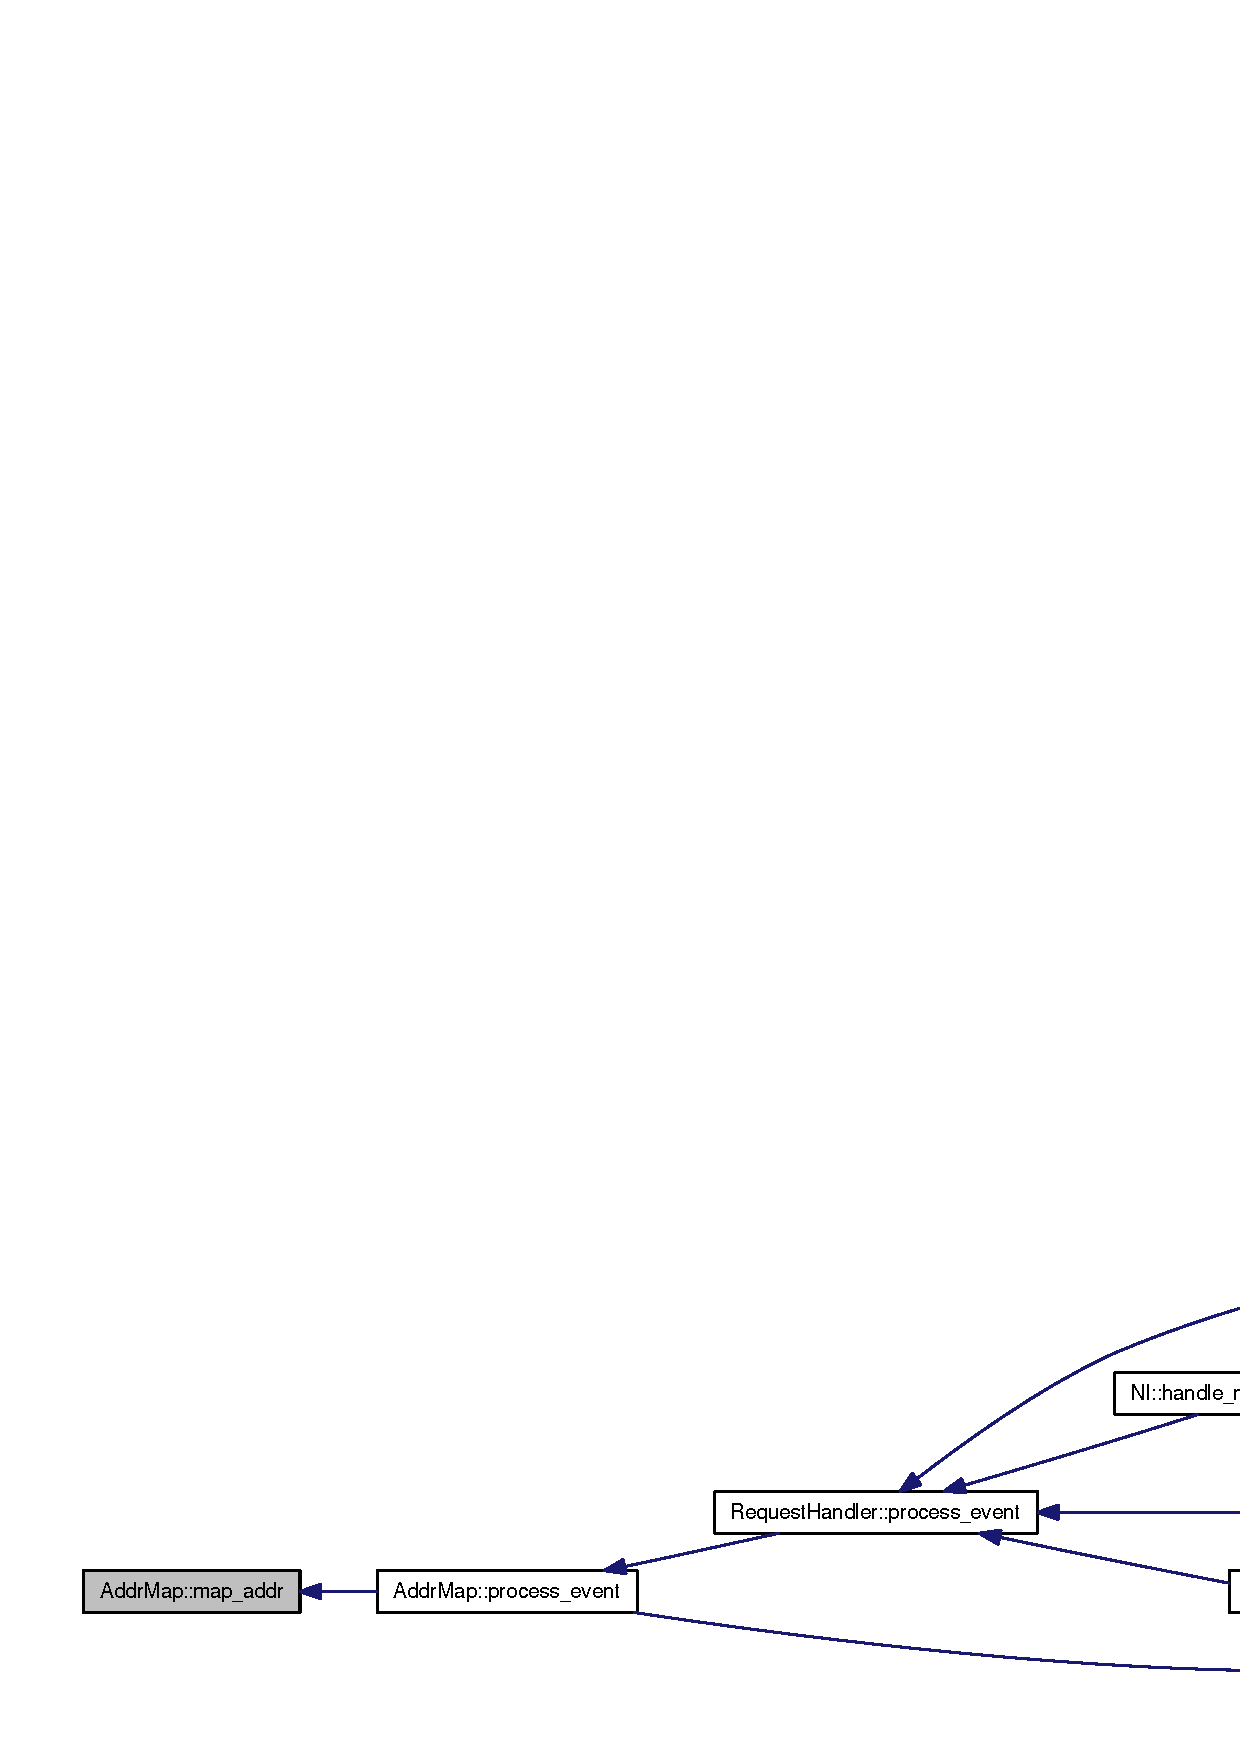
\includegraphics[width=420pt]{classAddrMap_0da8ea664e351b258473e04935d7170a_icgraph}
\end{center}
\end{figure}
\index{AddrMap@{AddrMap}!process\_\-event@{process\_\-event}}
\index{process\_\-event@{process\_\-event}!AddrMap@{AddrMap}}
\subsubsection[{process\_\-event}]{\setlength{\rightskip}{0pt plus 5cm}void AddrMap::process\_\-event ({\bf IrisEvent} $\ast$ {\em e})}\label{classAddrMap_e3ac527bcffced20f090db49c4047b60}


Main function that handles this class. 



Definition at line 58 of file addr\_\-map.cc.

References Request::address, Request::bankNo, Request::channelNo, Request::columnNo, map\_\-addr(), Simulator::Now(), parent, BankHandler::process\_\-event(), Request::rankNo, Request::rbufferInsertionTime, Request::rowNo, Simulator::Schedule(), and START.

Referenced by RequestHandler::process\_\-event().

Here is the caller graph for this function:\nopagebreak
\begin{figure}[H]
\begin{center}
\leavevmode
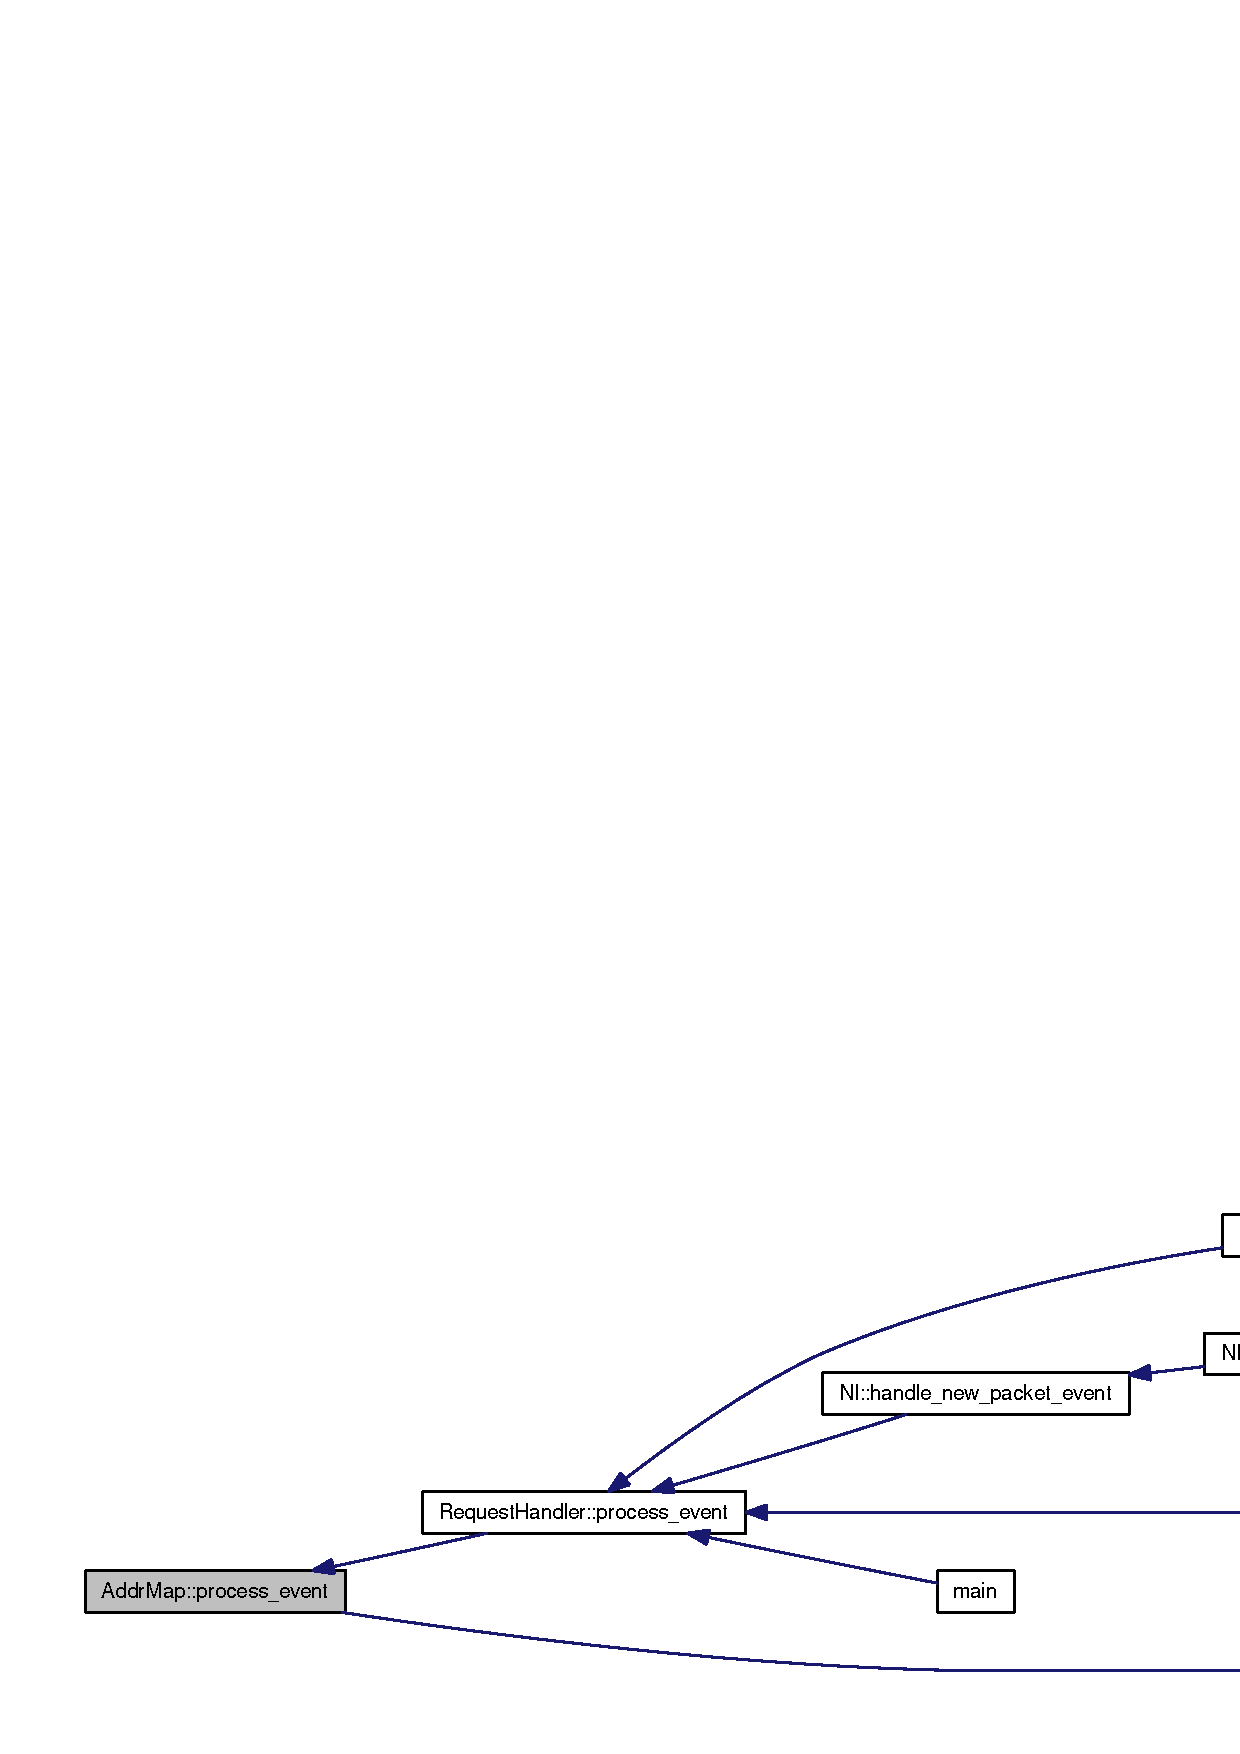
\includegraphics[width=420pt]{classAddrMap_e3ac527bcffced20f090db49c4047b60_icgraph}
\end{center}
\end{figure}
\index{AddrMap@{AddrMap}!toString@{toString}}
\index{toString@{toString}!AddrMap@{AddrMap}}
\subsubsection[{toString}]{\setlength{\rightskip}{0pt plus 5cm}std::string AddrMap::toString ()}\label{classAddrMap_4b0ee7e9842a671ec6ba76276f2f1feb}




Definition at line 116 of file addr\_\-map.cc.

\subsection{Member Data Documentation}
\index{AddrMap@{AddrMap}!parent@{parent}}
\index{parent@{parent}!AddrMap@{AddrMap}}
\subsubsection[{parent}]{\setlength{\rightskip}{0pt plus 5cm}{\bf Component}$\ast$ {\bf AddrMap::parent}}\label{classAddrMap_b0dc1ee5e15ff1f5e2cee9c3286b4f60}


pointer to the request handler 



Definition at line 49 of file addr\_\-map.h.

Referenced by process\_\-event(), and RequestHandler::RequestHandler().

The documentation for this class was generated from the following files:\begin{CompactItemize}
\item 
{\bf addr\_\-map.h}\item 
{\bf addr\_\-map.cc}\end{CompactItemize}
